\section{1985: RISCs}
Also on the hardware front, the world became more complex. Semiconductor
technology had made vast progress. It had become possible to place several
millions of transistors on one chip. Reduced size led to less signal propagation
time, and to higher speed. Designers were seduced to make use of the armies of
available transistors and include features that previously had been deferred to
software. A direct consequence were more on-chip registers, virtual addressing,
memory management units, and floating-point units. Apart from this, also
memories became bigger and faster, up to 1 MB per chip around 1985. Another
way to use up transistors was to offer a complex instruction set including string
instructions and those for decimal and for floating-point arithmetic. And yet another
was to offer a selection of addressing modes. The most advanced in this trend was
the 32000 series of National Semiconductor. Not only did it offer a set of address
length (similar to Lilith), but a large set of modes, including one for linking modules.
Besides, it was the first processor with 32-bit data paths. But compared to
conventional design with discrete components, computers based on these modern
chips (also Intel 80286 and Motorola 68000), were considered slow. The question
to which technology the future would belong was an open one.

The decision was made by the advent of Mosfet: Metal oxide semiconductor field
effect transistor. The gate is made conductive by electrons. In bipolar junction
transistors they are inserted by current injected into the gate layer between source
and drain, in FETs by applying a voltage to a layer isolated from the source-drain
channel, i.e. by a field effect. Today (2015) practically all transistors are FETs, and
the bipolar era has come to its end.

On the side of architecture, a complete revolution was taken shape. The trend
towards ever higher complexity was stopped. The new RISC excelled by simplicity.
Typically a processor now consisted of a set of registers (82 bits), and the
instruction set was minimized to simple logical and add/subtract instructions. Even
multiplication and division were left out. The rationale behind this departure from
conventions was that every instruction should require a single clock cycle and be
very fast. Code density became of negligible importance, because memory was
available in large amounts. If every instruction took a single cycle only, it became
possible to execute several instructions concurrently, each one in 4 - 5 steps:
Fetching, address computation (an addition), execution, and storing the result. This
concept was known as pipelining, and it promotes speed substantially.
\begin{figure}[h!]
  \centering
  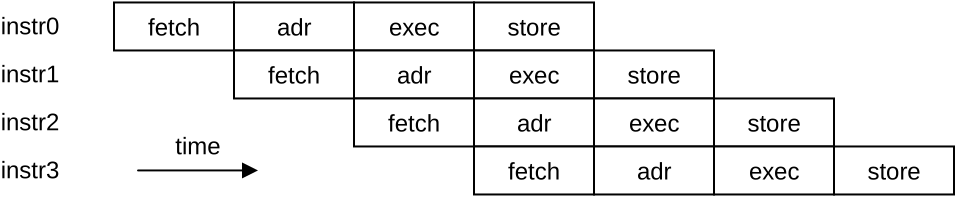
\includegraphics[width=\textwidth]{i/6}
\end{figure}

This scheme was proposed in academia (J. Hennessey at Stanford and D.
Patterson at Berkeley) around 1985. Start-up companies were the result: MIPS
and SPARC. In England similar developments evolved: Acorn at Cambridge,
leading to the ARM architecture. The ARM was the proponent that survived best.
However, as time went on, new versions appeared, each featuring new facilities
such as miniaturization of transistors would allow. Surprisingly, it could retain its
label even after its instruction set was practically replaced (by 16-bit "thumb"
instructions).
